Documento basado en muestra proporcionada por Prof. Toby Roberts (disponible \href{http://www.maths.adelaide.edu.au/anthony.roberts/LaTeX/Src/maths.tex}{aquí}).

\subsection{Análisis de la gráfica}
Hacer el estudio sobre una gráfica de una función consiste en analizar sus características a partir de lo que se observa en la gráfica. Para realizar este estudio, es necesario llevar a cabo, ordenadamente, los pasos que se indican en la siguiente tabla.\\
\begin{table}[]
	
	\begin{tabular}{|p{5cm}|}
		\hline
		\textbf{Formulario: características}\\ \hline
		\textbf{1. Tipo de función:} consiste en clasificar la función. \\ \hline
		\textbf{2. Dominio de una función:} conjunto de valores que toma la variable inependiente \textbf{x}. Se representa por \textbf{Dom(f)}.\\ \hline
		\textbf{3. Periodicidad de una función:} una función es periódica si se repite en intervalos iguales.\\ \hline
		\textbf{4. Simetría de una función:} se estudiarán sólo las simetrías respecto del origen O(0,0) y respecto del eje Y.\\ \hline
		\textbf{5. Asíntotas de una función:} rectas a las que se acerca la función en puntos muy alejados del origen sin llegar a tocarlas. Las asíntotas pueden ser verticales, horizontales y oblicuas. \\ \hline
		\textbf{6. Puntos de corte de una función con los ejes:} puntos en que $x=0$ y/o $y=0$. La gráfica puede cortar al eje X en varios puntos; al eje Y, como máximo, en uno.\newline \textbf{Signo:} intervalos del eje X en los que la función es positiva (+) o negativa (-). Las regiones están separadas por las abscisas de los puntos de corte del eje X y por las discontinuidades. \\ \hline
		\textbf{7. Máximos y mínimos relativos de una función:}\newline \textbf{Máximo relativo:} punto en el que el valor de la función es mayor que en los puntos que están muy cercanos.\newline \textbf{Mínimo relativo: } punto en que el valor de la función es menor que en los puntos que están muy cercanos.\newline \textbf{Monotonía: } consiste en estudiar en qué intervalos la función es creciente y en cuáles es decreciente. Los intervalos de crecimiento están separados por las abscisas de los máximos y mínimos relativos y por las discontinuidades. \\ \hline
		\textbf{8. Punto de inflexión de una función:} punto en que la función cambia de convexa $(\bigcup)$ a cóncava $(\bigcap)$ o viceversa, es decir, la recta tangente atraviesa a la gráfica.\newline \textbf{Curvatura:} consiste en estudiar en qué intervalos es convexa $(\bigcup)$ y en cuáles es cóncava $(\bigcap)$. Los intervalos de curvatura están separados por las abscisas de los puntos de inflexión y las discontinuidades.\\ \hline
		\textbf{9. Recorrido o imagen de una función:} conjunto de valores que toma la variable dependiente \textbf{y}. Se representa por \textbf{Im(f)}.\\ \hline
	\end{tabular}
	
\end{table}



\subsection{Clasificación de funciones}
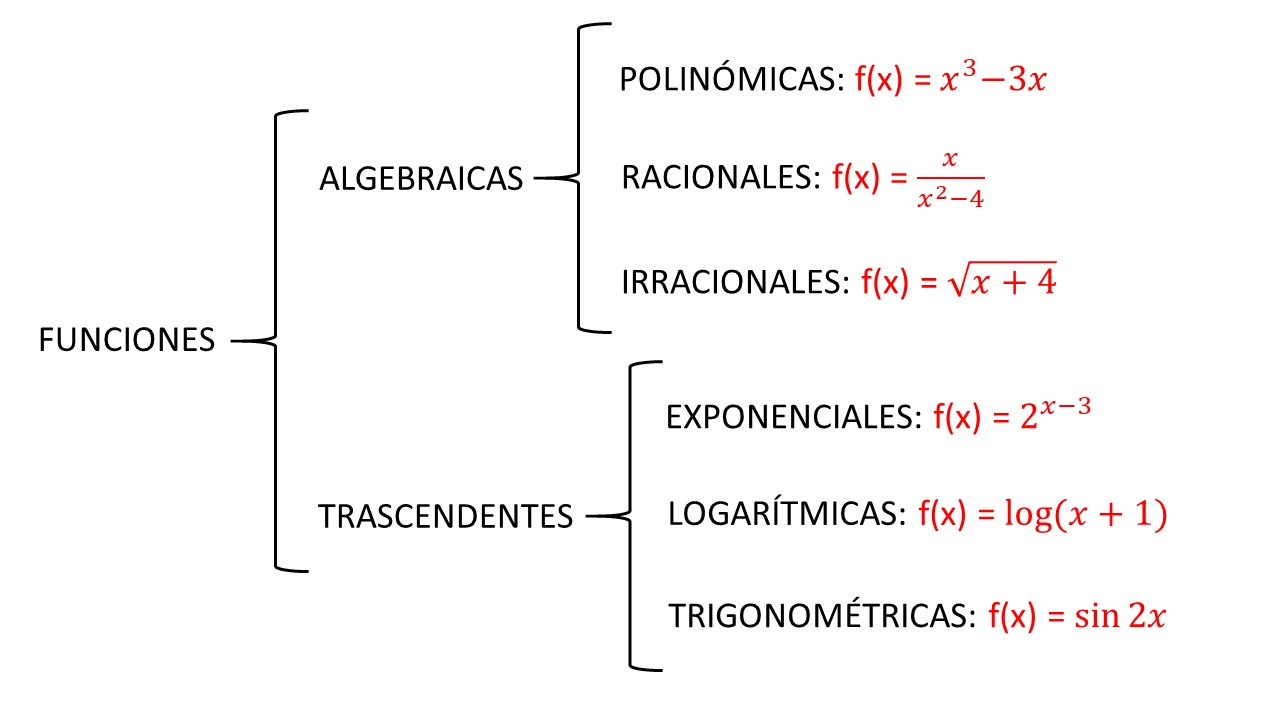
\includegraphics{samples/analisis/clasificaEsquema2.jpg}
\subsubsection{Ejemplos}
\begin{itemize}
	\item \textbf{Polinómicas.}
	$f(x) = x^3-3x$
	\geogebra{cwt7r5f7}
	\item \textbf{Racionales.}
	$f(x) = \dfrac{x}{x^2-4}$
	\geogebra{cdwjf88d}
	\item \textbf{Irracionales.}
	$f(x) = \sqrt{x+4}$
	\geogebra{xjn6vrn8}
	\item \textbf{Exponenciales.}
	$f(x) = 2^{x-3}$
	\geogebra{faj4urcm}
	\item \textbf{Logarítmicas.}
	$f(x) = \ln (x-1)$
	\geogebra{apzz89ae}
	\item \textbf{Trigonométricas.}
	$f(x) = \sin(2x)$
	\geogebra{yvw8jubg}
\end{itemize}

\subsection{Funciones polinómicas}
\youtube{YXUf8a3M9vk}
\subsubsection{Modelo de función polinómica}
Analiza y representa la función $y = 2x^2 - \dfrac{x^4}{4}$
\begin{itemize}
	\item \textbf{1. Tipo de función: }polinómica.
	\item \textbf{2. Dominio: }por ser una función polinómica, es toda la recta real $\mathbb{R}$ \\
	Dom(f) = $\mathbb{R} = (-\infty, +\infty)$.
	\item \textbf{3. Continuidad: }por ser polinómica, es toda la recta real $\mathbb{R}$.
	\item \textbf{4. Periodicidad: }no es periódica porque las funciones polinómicas nunca lo son.
	\item \textbf{5. Simetrías: }$f(-x)=2(-x)^2-\dfrac{(-x)^4}{4}=2x^2-\dfrac{x^4}{4}$\\ Se observa que $f(-x)=f(x) \rightarrow$ función par $\rightarrow$ simetría respecto del eje Y.
	\item \textbf{6. Asíntotas: }las funciones polinómicas no tienen asíntotas.
	\item \textbf{7. Corte con los ejes.}
	\begin{itemize}
	\item \textbf{Eje X: }$2x^2-\dfrac{x^4}{4}=0 \rightarrow x=0$, raíz doble; $x_1=2\sqrt{2}$, $x_2=-2\sqrt{2}$, raíces simples.\\
	Se obtienen los puntos $O(0,0)$, $A(-2\sqrt{2},0)$, $B(2\sqrt{2},0)$
	\item \textbf{Eje Y: }es el punto $O(0,0)$
	\item \textbf{Signo: }Si $x=1 \rightarrow f(1)=2-\dfrac{1}{4}=\dfrac{7}{4}>0$ (+)
	\end{itemize}
	\item \textbf{8. Máximos y mínimos:}\\
		$f'(x)=4x-x^3 \rightarrow 4x-x^3=0 \rightarrow x_1 = 0, x_2 = -2, x_3=2$, raíces simples.\\
		$f(x)=2x^2-\dfrac{x^4}{4}$\\
		\begin{itemize}
			\item $f(-2)=4 \rightarrow C(-2,4$)\\
			\item $f(0)=0 \rightarrow O(0,0)$\\
			\item $f(2)=4 \rightarrow D(2,4)$\\
		\end{itemize}
		$f''(x)=4-3x^2$
		\begin{itemize}
			\item $f''(-2)=-8 <0 \rightarrow C(-2,4)$ \textbf{máximo relativo}.\\
			\item $f''(0)=4 >0 \rightarrow O(0,0)$ \textbf{mínimo relativo}.\\
			\item $f''(2)=-8 <0 \rightarrow D(2,4)$ \textbf{máximo relativo}.\\
		\end{itemize}
		\textbf{Monotonía:}\\
		$f'(x)=4x-x^3 \rightarrow$ Si $x=1 \rightarrow f'(x)=4-1=3 > 0$ (+)
	\item \textbf{9. Puntos de inflexión:}\\
	$f''(x)= 4-3x^2 \rightarrow 4-3x^2=0 \rightarrow x_1= -\dfrac{2\sqrt{3}}{3}$, $x_2=\dfrac{2\sqrt{3}}{3}$ raíces simples.\\
	$f(x) = 2x^2-\dfrac{x^4}{4}$
	\begin{itemize}
		\item $f(-\dfrac{2\sqrt{3}}{3}) = \dfrac{20}{9} \rightarrow E(-\dfrac{2\sqrt{3}}{3}, \dfrac{20}{9})$
		\item $f(\dfrac{2\sqrt{3}}{3}) = \dfrac{20}{9} \rightarrow F(\dfrac{2\sqrt{3}}{3}, \dfrac{20}{9})$
	\end{itemize}
	$f'''(x)=-6x$
	\begin{itemize}
		\item $f'''(-\dfrac{2\sqrt{3}}{3}) = 4\sqrt{3} \neq 0 \rightarrow E(-\dfrac{2\sqrt{3}}{3}, \dfrac{20}{9})$, \textbf{punto de inflexión}.
		\item $f'''(\dfrac{2\sqrt{3}}{3}) = -4\sqrt{3} \neq 0 \rightarrow F(\dfrac{2\sqrt{3}}{3}, \dfrac{20}{9})$, \textbf{punto de inflexión}.
	\end{itemize}
	\item \textbf{10. Curvatura:}\\
	$f''(x)=4-3x^2 \rightarrow$ Si $x=0 \rightarrow f''(0)=4 > 0$ (+)
\end{itemize}
\geogebra{ceu6sks6}


\subsection{Funciones racionales}
\youtube{ARUEwJ_7sGc}
\subsubsection{Modelo de función racional}
Analiza y representa la función $y=\dfrac{x^3}{x^2-1}$
\begin{itemize}
	\item \textbf{1. Tipo de función: }racional.
	\item \textbf{2. Dominio: }por ser una función racional, hay que excluir las raíces del denominador: $x^2-1=0 \rightarrow x^2=1 \rightarrow x_1=-1$, $x_2=1$.\\
	$Dom(f) = \mathbb{R}-\{-1,1\} = (-\infty, -1) \bigcup (-1,1) \bigcup (1,+\infty)$
	\item \textbf{3. Continuidad: }es discontinua en $x=-1$, $x=1$, donde presenta discontinuidades de 1ª especie de salto finito.
	\item \textbf{4. Periodicidad: }no es periódica porque las funciones racionales nunca lo son.
	\item \textbf{5. Simetrías: }$f(-x)=\dfrac{(-x)^3}{(-x)^2-1}=\dfrac{-x^3}{x^2-1}=-\dfrac{x^3}{x^2-1}$\\
	Se observa que $f(-x) = -f(x) \rightarrow$ función impar $\rightarrow$ simetría respecto al origen $O(0,0)$
	\item \textbf{6. Asíntotas: }
	\begin{itemize}
		\item Verticales: son las raíces del denominador, $x=-1$, $x=1$\\
		Posición de la curva respecto a las asíntotas verticales:\\
		$$\lim_{x \to -1^{-}}(\dfrac{x^3}{x^2-1})=\dfrac{(-1^{-})^3}{(-1^{-})^2-1}=\dfrac{-1}{0^{+}}=-\infty$$
		$$\lim_{x \to -1^{+}}(\dfrac{x^3}{x^2-1})=\dfrac{(-1^{+})^3}{(-1^{+})^2-1}=\dfrac{-1}{0^{-}}=+\infty$$
		$$\lim_{x \to 1^{-}}(\dfrac{x^3}{x^2-1})=\dfrac{(1^{-})^3}{(1^{-})^2-1}=\dfrac{1}{0^{-}}=-\infty$$
		$$\lim_{x \to 1^{+}}(\dfrac{x^3}{x^2-1})=\dfrac{(1^{+})^3}{(1^{+})^2-1}=\dfrac{1}{0^{+}}=+\infty$$
		\item Horizontales: no tiene.
		\item Oblicuas: $y=x$\\
		Posición de la curva respecto de la asíntota oblicua:
		$$\lim_{x \to -\infty}(\dfrac{x}{x^2-1})=\dfrac{-\infty}{(-\infty)^2-1}=0^{-}$$
		$$\lim_{x \to +\infty}(\dfrac{x}{x^2-1})=\dfrac{+\infty}{(+\infty)^2-1}=0^{+}$$
	\end{itemize}
	\item \textbf{7. Corte con los ejes:}
	\begin{itemize}
		\item \textbf{Eje X: }$x^3=0 \rightarrow x=0$ raíz triple. Se obtiene el punto $O(0,0)$.
		\item \textbf{Eje Y: }el punto $O(0,0)$.
		\item \textbf{Signo: }Si $x=2 \rightarrow f(2)=\dfrac{2^3}{2^2-1}=\dfrac{8}{3}>0$(+)
	\end{itemize}
	\item \textbf{8. Máximos y mínimos relativos:}\\
	$x^2(x^2-3)=0 \rightarrow x=0 $raíz doble; $x=-\sqrt{3}$, $x=\sqrt{3}$ raíces simples.\\
	$f''(-\sqrt{3})=-\dfrac{3\sqrt{3}}{2}<0 \rightarrow A(-\sqrt{3}, -\dfrac{3\sqrt{3}}{2})$, \textbf{máximo relativo}.\\
	$f''(\sqrt{3})=\dfrac{3\sqrt{3}}{2}>0 \rightarrow B(\sqrt{3}, \dfrac{3\sqrt{3}}{2})$, \textbf{mínimo relativo}.\\
	\textbf{Monotonía: }\\
	$f'(x)=\dfrac{x^4-3x^2}{(x^2-1)^2} \rightarrow$ Si $x=2 \rightarrow f'(2)=\dfrac{2^4-3 \cdot 2^2}{(2^2-1)^2}=\dfrac{4}{9}>0$(+)\\
	Las raíces del denominador son discontinuidades dobles.
	\item \textbf{9. Puntos de inflexión:}\\
	$2x(x^2+3) = 0 \rightarrow x=0$ raíz simple.\\
	$f'''(x) = - \dfrac{6x^4+36x^2+6}{(x^2-1)^4} \rightarrow f'''(0)=-6 \neq 0 \rightarrow O(0,0)$, \textbf{punto de inflexión}.\\
	\textbf{Curvatura:}\\
	$f''(x)=\dfrac{2x^3+6x}{(x^2-1)^3} \rightarrow$ Si $x=2 \rightarrow f''(2)=\dfrac{2 \cdot 2^3+6 \cdot 6}{(2^2-1)^3}=\dfrac{28}{27}>0$(+)\\
	Las raíces del denominador son discontinuidades triples.
	
\end{itemize}
\geogebra{s2j8hxtz}

\subsection{Funciones irracionales}
\youtube{akSVuDk_lhw}
\subsubsection{Modelo de función irracional}
Analiza y representa la función $y=\sqrt{x^2-4}$
\begin{itemize}
	\item \textbf{1. Tipo de función: }irracional.
	\item \textbf{2. Dominio: }por ser una función irracional de índice par, el radicando tiene que ser mayor o igual que cero.\\
	$x^2-4 \geq 0$, se resuelve la ecuación correspondiente $x^2-4=0 \rightarrow x^2=4 \rightarrow x_1=-2$, $x_2=2$. Como las raíces son simples, $x^2-4$ cambia de signo en cada una de ellas.\\
	Dom(f)= $(-\infty, -2] \bigcup [2, +\infty)$
	\item \textbf{3. Continuidad: }es discontinua en $x=-2$, $x=2$.
	\begin{itemize}
		\item Para $x=-2$, se tiene $f(-2)=0$:
		$$\lim_{x \to -2^{-}}(\sqrt{x^2-4})=0$$
		$$\lim_{x \to -2^{+}}(\sqrt{x^2-4}) \text{no existe}$$
		Por tanto, para $x=-2$, la función tiene una discontinuidad de 2ª especie.\\
		\item Para $x=-2$, se tiene $f(-2)=0$:
		$$\lim_{x \to 2^{-}}(\sqrt{x^2-4}) \text{no existe}$$
		$$\lim_{x \to 2^{+}}(\sqrt{x^2-4})=0$$
		Por tanto, para $x=2$, la función tiene una discontinuidad de 2ª especie.\\
	\end{itemize}
	\item \textbf{4. Periodicidad: }no es periódica. Las funciones irracionales nunca lo son.
	\item \textbf{5. Simetrías: }$f(-x) = \sqrt{(-x)^2-4} = \sqrt{x^2-4}$\\
	Se observa que $f(-x)=f(x) \rightarrow $función par $\rightarrow$ simétrica respecto al eje Y.
	\item \textbf{6. Asíntotas: }
	\begin{itemize}
		\item Verticales: no tiene.
		\item Horizontales: no tiene.
		\item Oblicuas: presenta asíntotas oblicuas en $y=x$ y en $y=-x$.
	\end{itemize}
	\item \textbf{7. Corte con los ejes: }
	\begin{itemize}
		\item \textbf{Eje X: }$\sqrt{x^2-4} = 0 \rightarrow x^2-4=0 \rightarrow x^2=4 \rightarrow x_1=-2$, $x_2=2$\\
		Se obtienen los puntos $A(-2, 0)$ y $B(2,0)$
		\item \textbf{Eje Y: }no lo corta.
		\item \textbf{Signo: }Si $x=3 \rightarrow f(3)=\sqrt{3^2-4}=\sqrt{9-4}=\sqrt{5}>0$ (+)
	\end{itemize}
	\item \textbf{8. Máximos y mínimos relativos: }
	$f'(x)=\dfrac{x}{\sqrt{x^2-4}} \rightarrow x=0 \notin$ Dom(f)\\
	No tiene ni máximos ni mínimos relativos.\\
	\textbf{Monotonía: }si $x=3 \rightarrow f'(3)=\dfrac{3}{\sqrt{3^2-4}}=\dfrac{3}{\sqrt{5}}>0$ (+)
	\item \textbf{9. Puntos de inflexión: }\\
	$f''(x)=-\dfrac{4}{(x^2-4)\sqrt{x^2-4}}$ \\
	$f''(x)$ nunca se hace cero, por lo tanto no ha puntos de inflexión.\\
	\textbf{Curvatura: }si $x=3 \rightarrow f''(3)=-\dfrac{4}{(3^2-4)\sqrt{3^2-4}}=-\dfrac{4}{5\sqrt{5}}<0$ (-)	
\end{itemize}
\geogebra{nxe84yaw}

\subsection{Funciones exponenciales}
\youtube{JulYyOS0hH4}
\subsubsection{Modelo de función exponencial}
Analiza y representa la función $y=(2-x)e^x$
\begin{itemize}
	\item \textbf{1. Tipo de función: }producto de polinómica por exponencial.
	\item \textbf{2. Dominio: }por ser el producto de una función polinómica por una función exponencial, es toda la recta real $\mathbb{R}$.\\
	Dom(f) = $\mathbb{R}=(-\infty, +\infty)$
	\item \textbf{3. Continuidad: }por ser el producto de una función polinómica por una exponencial, es continua en toda la recta real $\mathbb{R}$. 
	\item \textbf{4. Periodicidad: }no es periódica, ya que las funciones polinómicas y exponenciales nunca lo son.
	\item \textbf{5. Simetrías: }$f(-x)=(2+x)e^{-x}$\\
	Se observa que $f(-x)\neq f(x)$, $f(-x) \neq -f(x) \rightarrow$ no es simétrica ni respecto al eje Y ni respecto del orien $O(0,0)$.
	\item \textbf{6. Asíntotas: }\\
	\begin{itemize}
		\item Verticales: no tiene.
		\item Horizontales: \\
		$$\lim_{x \to -\infty}((2-x)e^x)=0$$
		$$\lim_{x \to +\infty}((2-x)e^x)=-\infty$$
		Asíntota horizontal $y=0$, pero sólo por la izquierda.\\
		Posición de la curva respecto de la asíntota oblicua:
		$$\lim_{x \to -\infty}((2-x)e^x)=0^{+}$$
		La curva está encima de la asíntota.
		\item Oblicuas: no tiene.
	\end{itemize}
	\item \textbf{7. Corte con los ejes: }
	\begin{itemize}
		\item \textbf{Eje X: }$(2-x)e^{x} = 0 \rightarrow x=2$, raíz simple. Se obtiene el punto $A(2,0)$.
		\item \textbf{Eje Y: }es el punto $B(0,2)$.
		\item \textbf{Signo: }Si $x=0 \rightarrow f(0)=2 >0$ (+)
	\end{itemize}
	\item \textbf{8. Máximos y mínimos relativos: }\\
	$f'(x)=(1-x)e^x \rightarrow (1-x)e^x = 0 \rightarrow x=1$, raíz simple.\\
	$f(x)=(2-x)e^x \rightarrow f(1)=e \rightarrow C(1,e)$\\
	$f''(x)=-ze^{x} \rightarrow f''(x)=-e < 0 \rightarrow C(1,e)$, \textbf{máximo relativo}.\\
	\textbf{Monotonía: }\\
	$f''(x)=(1-x)e^x \rightarrow $Si $x=0 \rightarrow f'(0) = 1>0$ (+) 
	\item \textbf{9. Puntos de inflexión:}\\
	$f''(x)=-xe^x \rightarrow -xe^x = 0 \rightarrow x=0$, raíz simple.\\
	$f(x)=(2-x)e^x \rightarrow f(0)=2 \rightarrow B(0,2)$\\
	$f'''(x)=-(x+1)e^x \rightarrow f'''(0)=-1 \neq 0 \rightarrow B(0,2)$, \textbf{punto de inflexión}.\\
	\textbf{Curvatura:}\\
	$f''(x)=-xe^x \rightarrow $si $x=1 \rightarrow f''(1)=-e<0$ (-)
	
\end{itemize}
\geogebra{cthuzvhc}

\subsection{Funciones logarítmicas}
\youtube{a7mRvMyayVM}
\subsubsection{Modelo de función logarítmica}
Analiza y representa la función $y=\ln (x^2-1)$
\begin{itemize}
	\item \textbf{1. Tipo de función: }logarítmica.
	\item \textbf{2. Dominio: }por ser una función logarítmica, el argumento tiene que ser positivo, es decir, mayor que cero.\\
	$x^2-1 >0$, se resuelve la ecuación correspondiente $x^2-1 = 0 \rightarrow x^2=1 \rightarrow x_1=-1$, $x_2=1$. Como las raíces son simples, en cada una de ellas $x^2-1$ cambia el signo.\\
	$x^2-1 \rightarrow $Si $x=0 \rightarrow 0^2-1 = -1 <0$ (-)\\
	Dom(f)=$(-\infty , -1)\bigcup(1, +\infty)$
	\item \textbf{3. Continuidad: }es discontinua en $x=-1, x=1$
	\begin{itemize}
		\item Para $x=-1$, se tiene $f(-1)$ no existe:\\
		$$\lim_{x \to -1^{-}}(\ln (x^2-1))=-\infty$$
		$$\lim_{x \to -1^{+}}(\ln (x^2-1)) \text{no existe}$$
		Por tanto, para $x=-1$, la función tiene una discontinuidad de 2ª especie.
		\item Para $x=1$, se tiene $f(1)$ no existe:\\
		$$\lim_{x \to 1^{-}}(\ln (x^2-1)) \text{no existe}$$
		$$\lim_{x \to 1^{+}}(\ln (x^2-1))=-\infty$$
		Por tanto, para $x=1$, la función tiene una discontinuidad de 2ª especie.
	\end{itemize}
	\item \textbf{4. Periodicidad: }no es periódica, porque las funciones logarítmicas nunca lo son.
	\item \textbf{5. Simetrías: }$f(-x)= \ln[(-x)^2-1] = \ln(x^2-1)$\\
	Se observa que $f(-x)=f(x) \rightarrow$ función par $\rightarrow$ simetría respecto del eje Y.
	\item \textbf{6. Asíntotas: }
	\begin{itemize}
		\item Verticales: $x=-1, x=1$\\
		Posición de la curva respecto de las asíntotas verticales:
		$$\lim_{x \to -1^{-}}(\ln (x^2-1))=-\infty$$
		$$\lim_{x \to -1^{+}}(\ln (x^2-1)) \text{no existe}$$
		$$\lim_{x \to 1^{-}}(\ln (x^2-1)) \text{no existe}$$
		$$\lim_{x \to 1^{+}}(\ln (x^2-1))=-\infty$$
		\item Horizontales: no tiene.
		\item Oblicuas: no tiene.
	\end{itemize}
	\item \textbf{7. Corte con los ejes: }
	\begin{itemize}
		\item \textbf{Eje X: }$\ln(x^2-1) = 0 \rightarrow x^2-1=1 \rightarrow x^2=2 \rightarrow x_1=-\sqrt{2}$, $x_2=\sqrt{2}$, raíces simples. Se obtienen los puntos $A(-\sqrt{2},0); B(\sqrt{2},0)$\\
		Se obtienen los puntos $A(-2, 0)$ y $B(2,0)$
		\item \textbf{Eje Y: }no lo corta.
		\item \textbf{Signo: }Si $x=2 \rightarrow f(2)=\ln(3)>0$ (+)
	\end{itemize}
	\item \textbf{8. Máximos y mínimos relativos: }\\
	$f'(x)=\dfrac{2x}{x^2-1} \rightarrow \dfrac{2x}{x^2-1} = 0 \rightarrow x=0 \notin$ Dom(f)\\
	No tiene ni máximos ni mínimos relativos.\\
	\textbf{Monotonía: }\\
	$f'(x) = \dfrac{2x}{x^2-1} \rightarrow $Si $x=2 \rightarrow f'(2)=\dfrac{2\cdot 2}{2^2-1} = \dfrac{4}{3}>0$ (+)
	\item \textbf{9. Puntos de inflexión: }\\
	$f''(x)=-\dfrac{2x^2+2}{(x^2-1)^{2}}$ \\
	$f''(x)$ nunca se hace cero, por lo tanto no ha puntos de inflexión.\\
	\textbf{Curvatura: }\\
	$f''(x)=-\dfrac{2x^2+2}{(x^2-1)^{2}}$ siempre es negativo $\rightarrow$ siempre es cóncava $(\bigcap)$.	
\end{itemize}
\geogebra{pgghxa8t}

\subsection{Funciones trigonométricas}
\subsubsection{Modelo de función trigonométrica}
Analiza y representa la función $y=3 \sin 2x$
\begin{itemize}
	\item \textbf{1. Tipo de función: }trigonométrica.
	\item \textbf{2. Dominio: }las funciones seno y coseno están definidas en todos los números reales $\mathbb{R}$.\\
	Dom(f) = $\mathbb{R}=(-\infty, +\infty)$
	\item \textbf{3. Periodicidad: }es periódica en, de período $\dfrac{2\pi}{2} = \pi$\\
	Solo la estudiaremos en el primer período positivo $[0, \pi)$
	\item \textbf{4. Simetrías: }$f(-x) = 3 \sin (-2x) = -3 \sin (2x)$\\
	Se observa que $f(-x)=-f(x) \rightarrow$ función impar $\rightarrow$ simétrica respecto al origen de coordenadas $O(0,0)$.
	\item \textbf{5. Asíntotas: }
	\begin{itemize}
		\item Verticales: no tiene.
		\item Horizontales: no tiene.
		\item Oblicuas: no tiene.
	\end{itemize}
	\item \textbf{6. Corte con los ejes: }
	\begin{itemize}
		\item \textbf{Eje X: }$3\sin(2x)=0 \rightarrow \sin(2x) = 0 \rightarrow x_1=0$, $x_2=\dfrac{\pi}{2}$, raíces simples; Se obtienen los puntos $O(0,0); A(\dfrac{\pi}{2}, 0)$.\\
		\item \textbf{Eje Y: }es el punto $O(0,0)$
		\item \textbf{Signo: }Si $x=\dfrac{\pi}{4} \rightarrow f(\dfrac{\pi}{4})=3\cdot \sin(\dfrac{2\pi}{4}) = 3 \sin(\dfrac{\pi}{2})>0$ (+)
	\end{itemize}
	\item \textbf{7. Máximos y mínimos: }\\
	\begin{itemize}
		\item $B(\dfrac{\pi}{4}, 3)$, \textbf{máximo relativo}
		\item $C(\dfrac{3\pi}{4}, -3)$, \textbf{mínimo relativo}.
	\end{itemize}
	\textbf{Monotonía: }\\
	\begin{itemize}
		\item Creciente: $(0, \dfrac{\pi}{4}) \bigcup (\dfrac{3\pi}{4}, \pi))$
		\item Decreciente: $(\dfrac{\pi}{4}, \dfrac{3\pi}{4})$
	\end{itemize}
	\item \textbf{8. Puntos de inflexión:}\\
	\begin{itemize}
		\item $O(0,0)$, \textbf{punto de inflexión}.
		\item $A(\dfrac{\pi}{2},0)$, \textbf{punto de inflexión}.
	\end{itemize}
	\textbf{Curvatura: }\\
	\begin{itemize}
		\item Convexa $(\bigcup)$: $(\dfrac{\pi}{2}, \pi)$.
		\item Cóncava $(\bigcap)$: $(0, \dfrac{\pi}{2})$
	\end{itemize}
\end{itemize}
\geogebra{jufgczka}
\subsubsection{Ejercicios}
\begin{ex}[sol later]
	Ayudándote del panel, representa gráficamente las tres funciones trigonométricas más conocidas y observa las diferencias.
	\geogebra[ai=true, stb=true]{tc5pbmae}
	\begin{sol}
		Las funciones que se deben representar son el coseno, el seno y la tangente.
	\end{sol}
\end{ex}

